\definecolor{lgry}{RGB}{188,188,188}
\definecolor{dgry}{RGB}{150,150,150}

\makeatletter

\tikzstyle{chart}=[
    legend label/.style={font={\scriptsize},anchor=west,align=left},
    legend box/.style={rectangle, draw, minimum size=5pt},
    axis/.style={black,semithick,->},
    axis label/.style={anchor=east,font={\tiny}},
]

\tikzstyle{pie chart}=[
    chart,
    slice/.style={line cap=round, line join=round, very thick,draw=black},
    pie title/.style={font={\bf}},
    slice type/.style 2 args={
        ##1/.style={fill=##2},
        values of ##1/.style={}
    }
]

\pgfdeclarelayer{background}
\pgfdeclarelayer{foreground}
\pgfsetlayers{background,main,foreground}


\newcommand{\pie}[3][]{
    \begin{scope}[#1]
    \pgfmathsetmacro{\curA}{90}
    \pgfmathsetmacro{\r}{1}
    \def\c{(0,0)}
    \node[pie title] at (90:1.3) {#2};
    \foreach \v/\s in{#3}{
        \pgfmathsetmacro{\deltaA}{\v/100*360}
        \pgfmathsetmacro{\nextA}{\curA + \deltaA}
        \pgfmathsetmacro{\midA}{(\curA+\nextA)/2}

        \path[slice,\s] \c
            -- +(\curA:\r)
            arc (\curA:\nextA:\r)
            -- cycle;
        \pgfmathsetmacro{\d}{max((\deltaA * -(.5/50) + 1) , .5)}

        \begin{pgfonlayer}{foreground}
        \path \c -- node[pos=\d,pie values,values of \s]{$\v\%$} +(\midA:\r);
        \end{pgfonlayer}

        \global\let\curA\nextA
    }
    \end{scope}
}

\newcommand{\legend}[2][]{
    \begin{scope}[#1]
    \path
        \foreach \n/\s in {#2}
            {
                  ++(0,-10pt) node[\s,legend box] {} +(5pt,0) node[legend label] {\n}
            }
    ;
    \end{scope}
}

\section{Foug\`ere: a data dissemination library}

\begin{frame}{Foug\`ere Overview}
    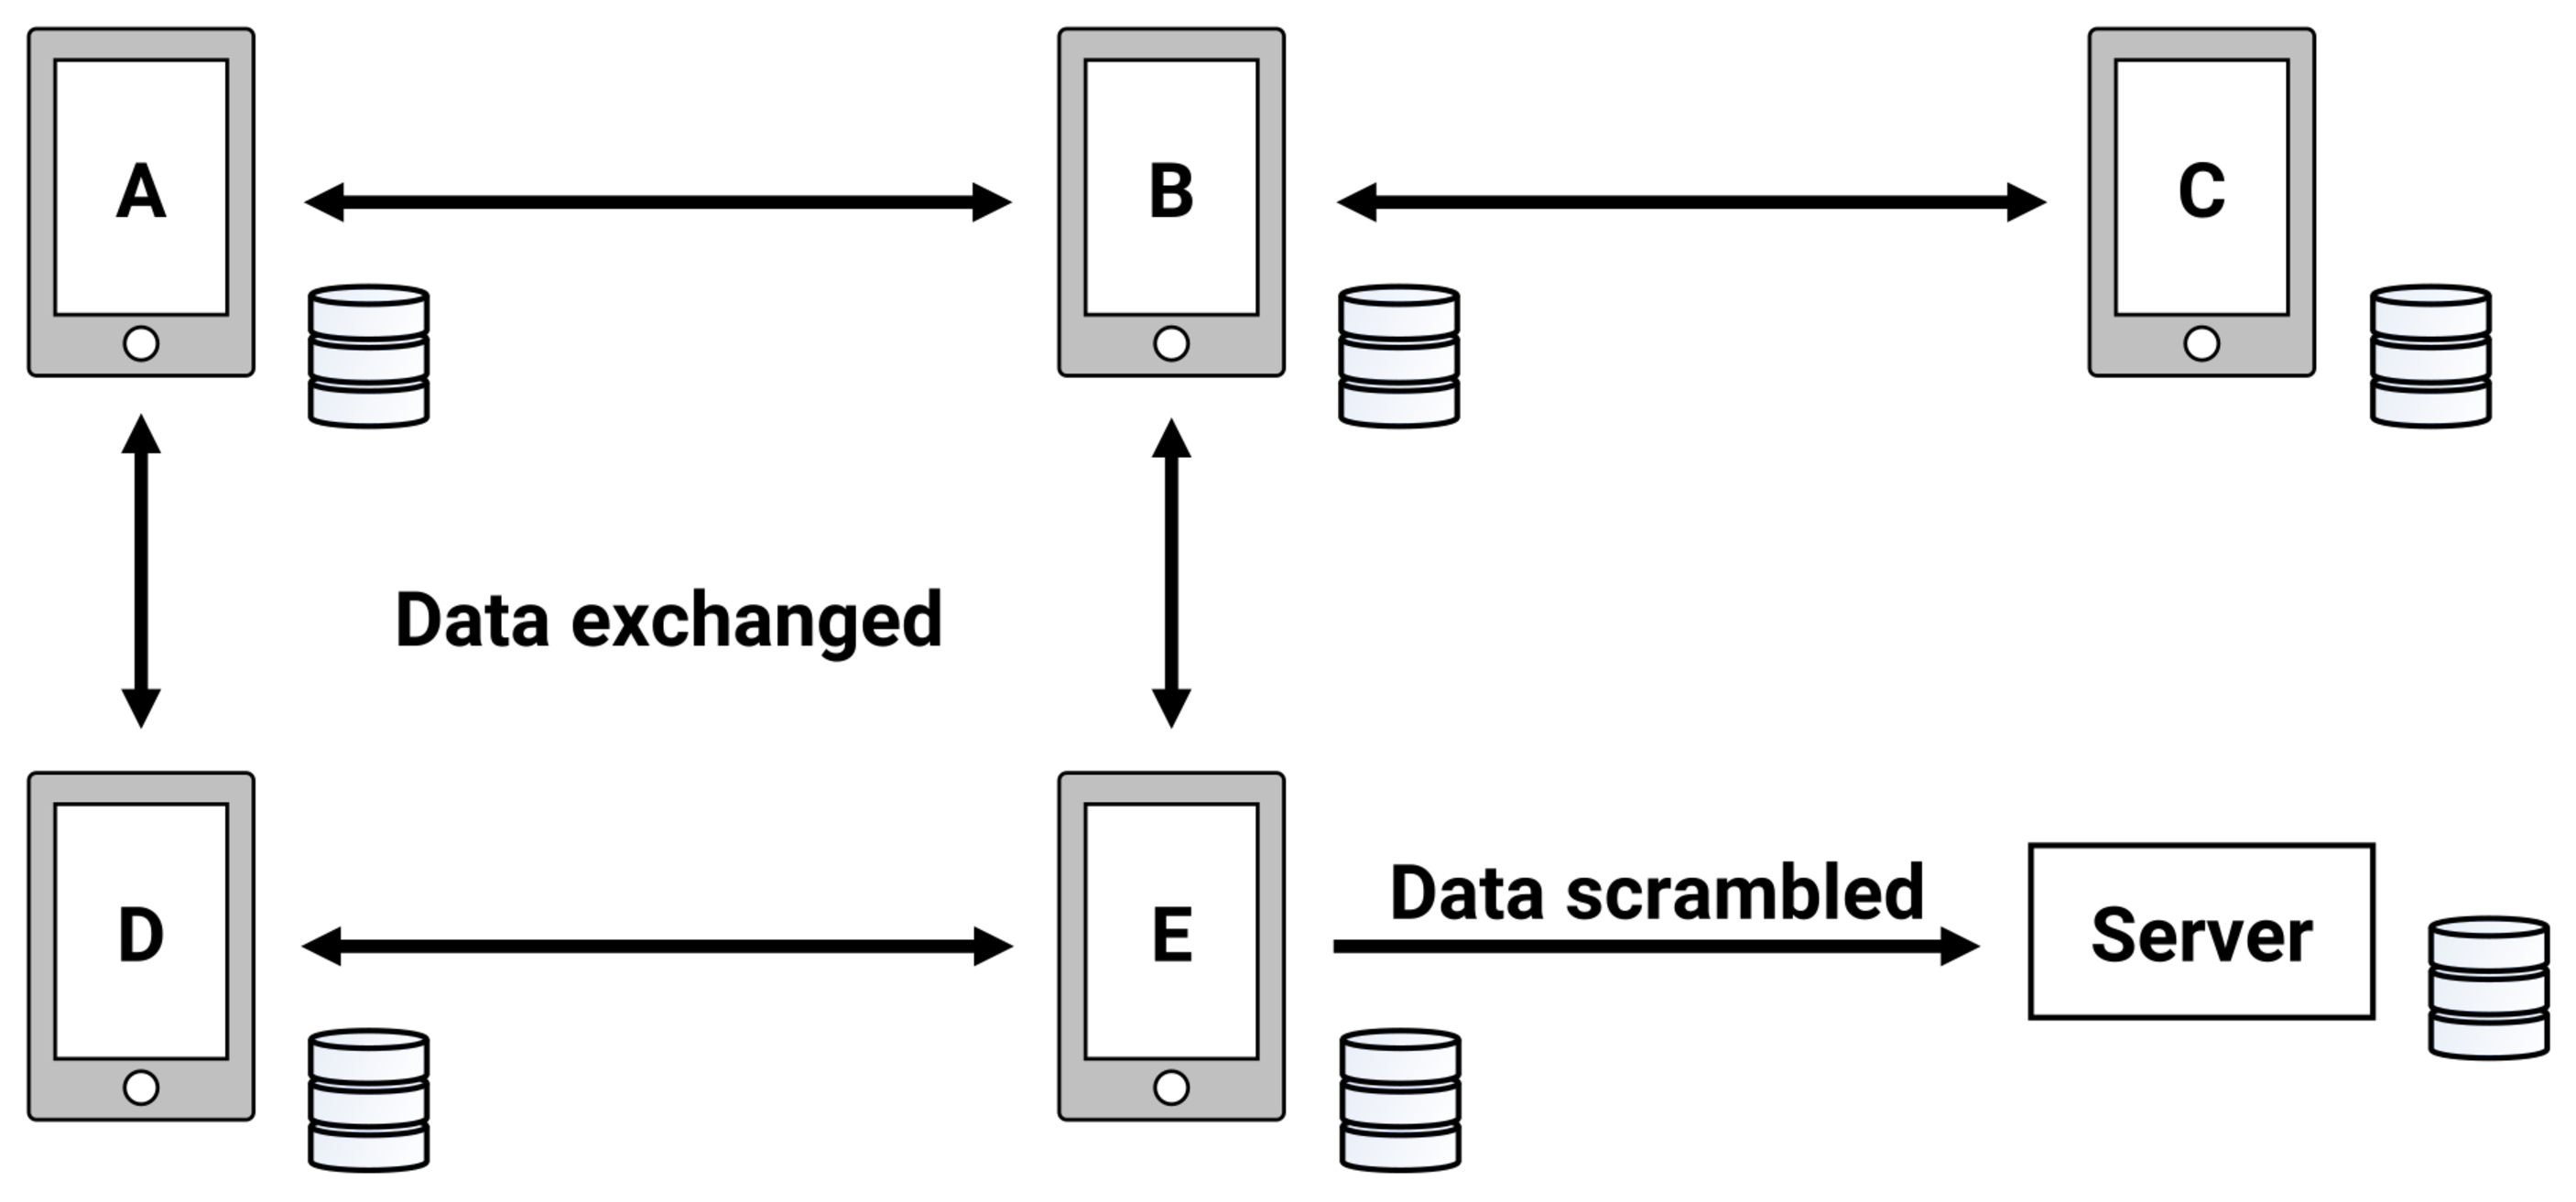
\includegraphics[width=\textwidth]{figures/wifidirect}
\end{frame}

\begin{frame}{Foug\`ere Principles}
    Foug\`ere includes 3 different types of neighbors:
    \begin{itemize}
        \item \textit{Physical}
        \item \textit{Social}
        \item \textit{Contextual}
    \end{itemize}
\end{frame}

\begin{frame}{Dissemination}
  \begin{figure}[<+->]
    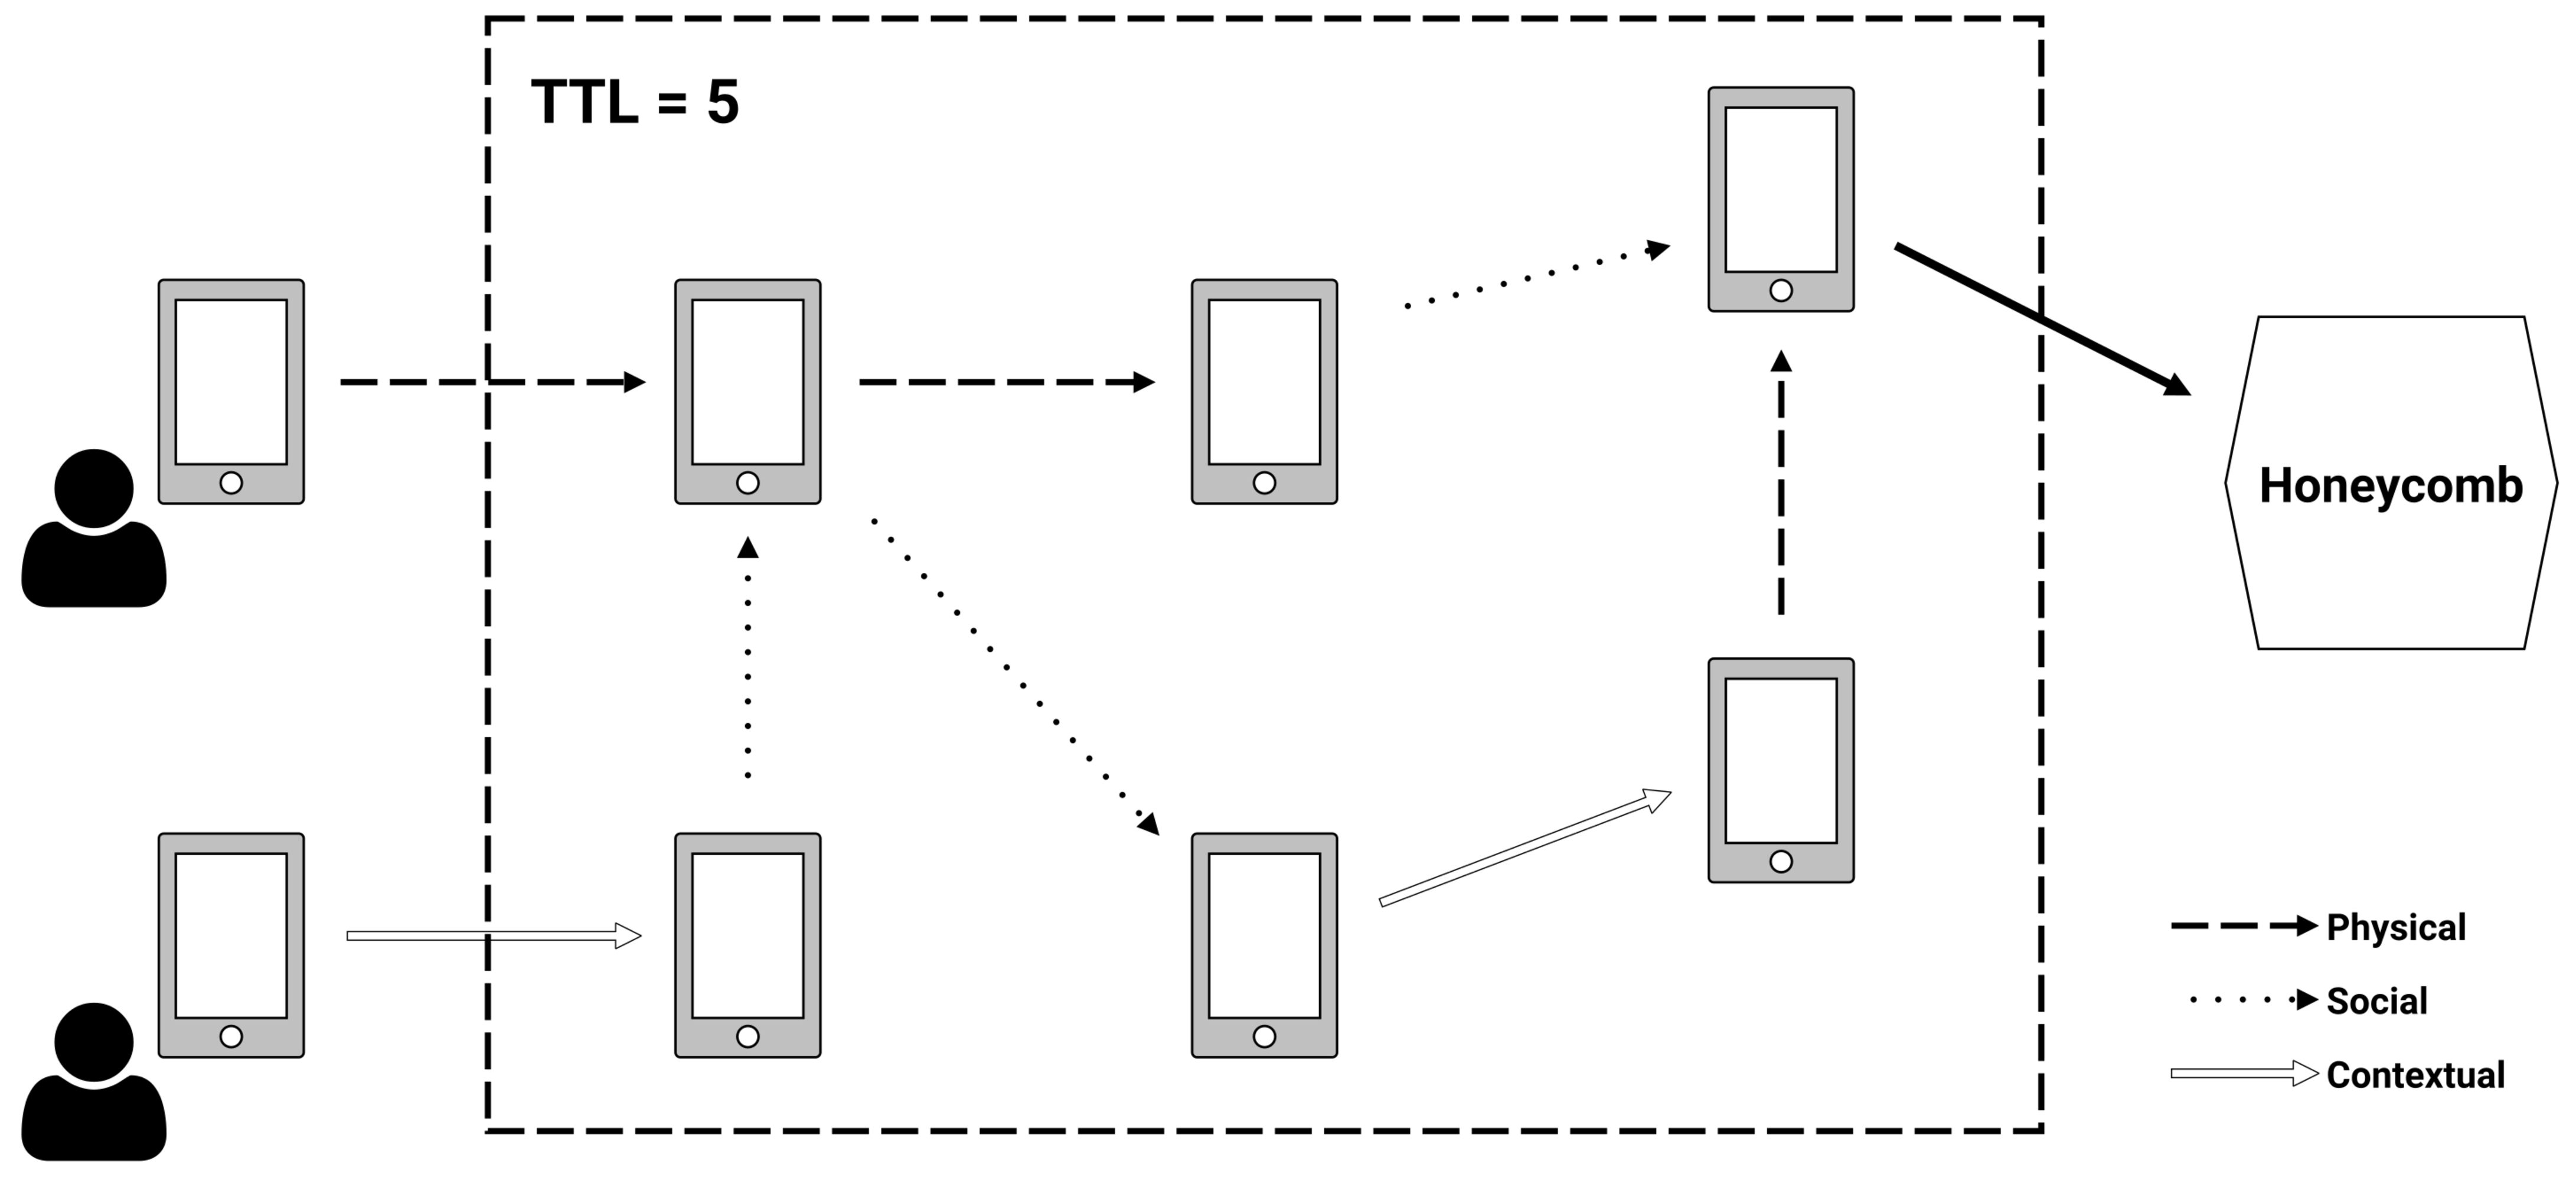
\includegraphics[width=\textwidth]{figures/ttl}<1>
    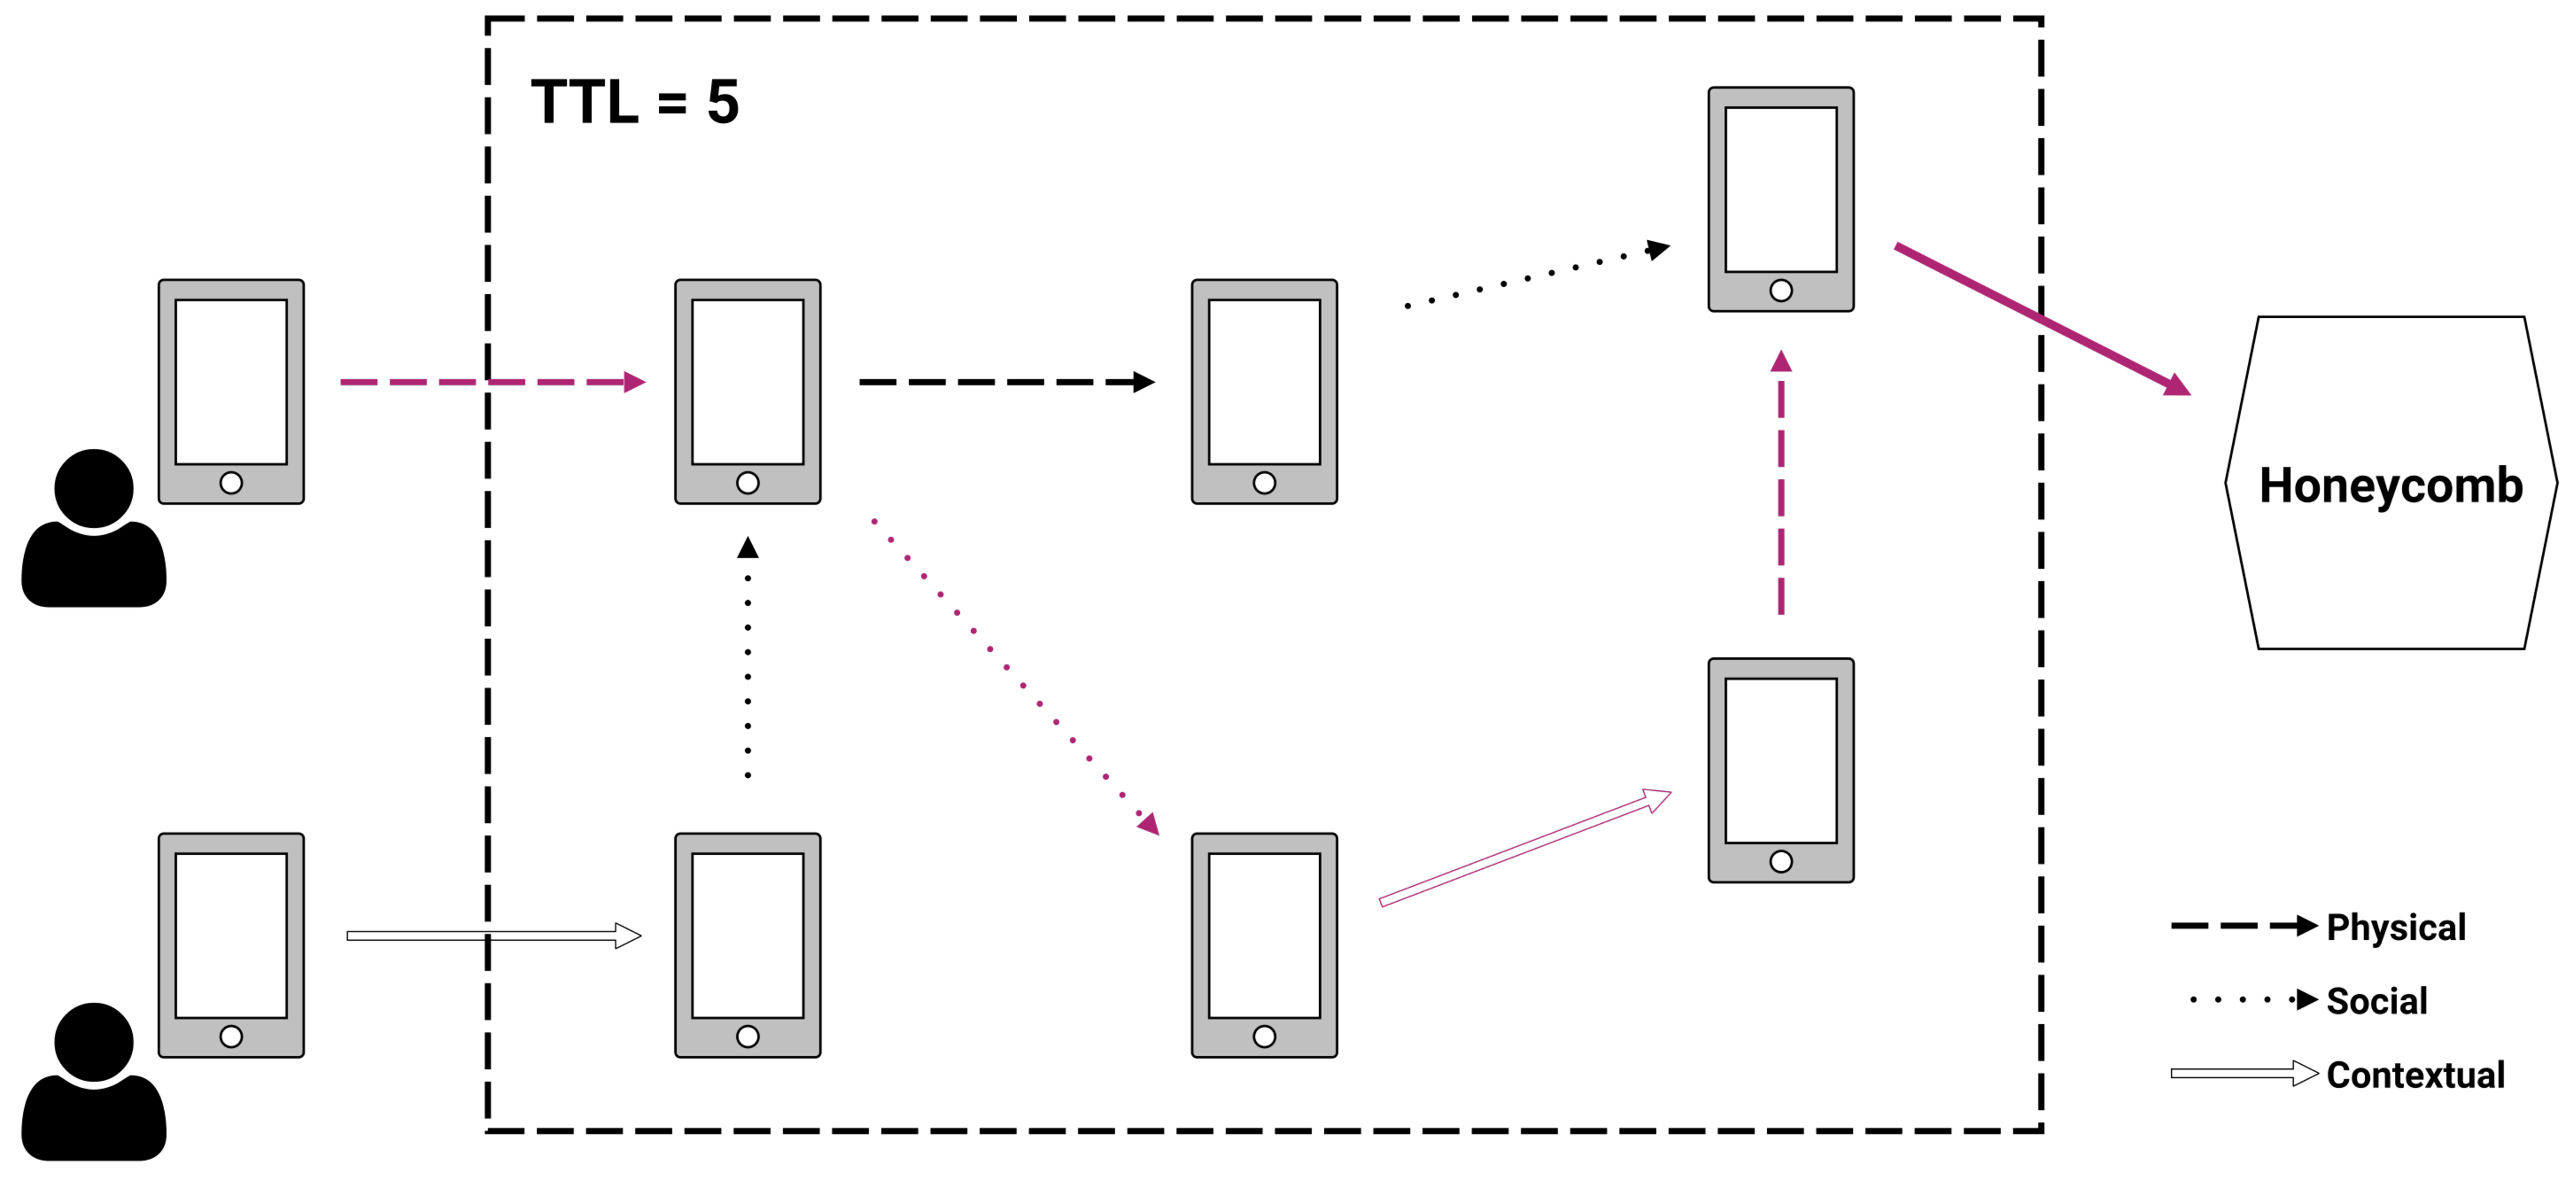
\includegraphics[width=\textwidth]{figures/ttl1}<2>
    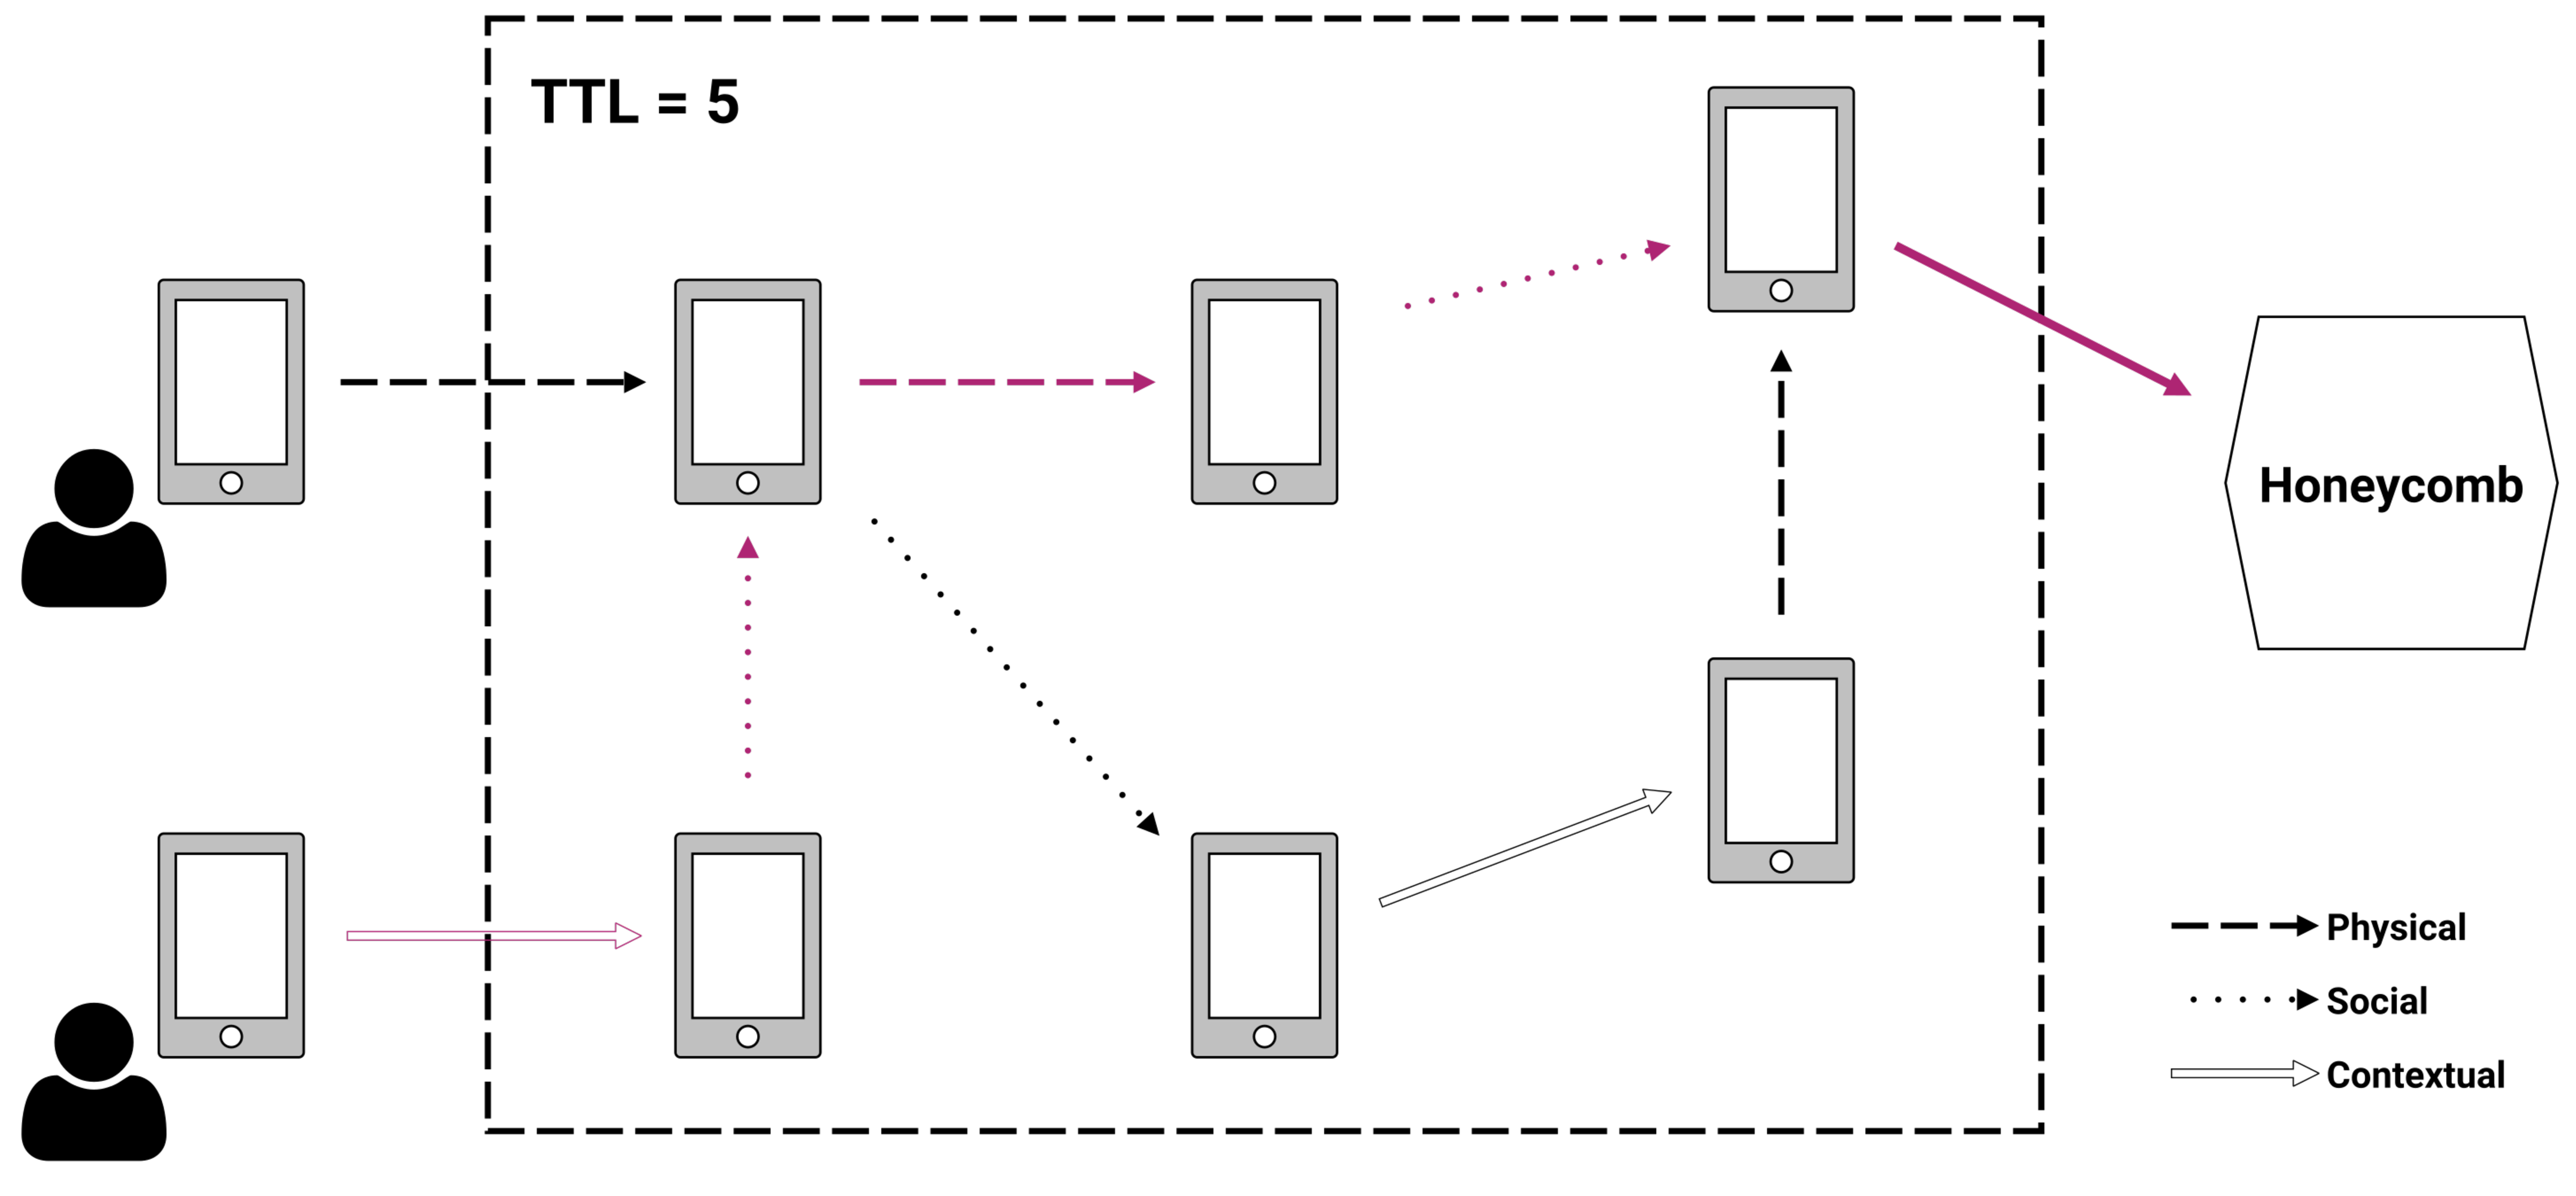
\includegraphics[width=\textwidth]{figures/ttl2}<3>
  \end{figure}
\end{frame}

\begin{frame}{Foug\`ere Implementation}
    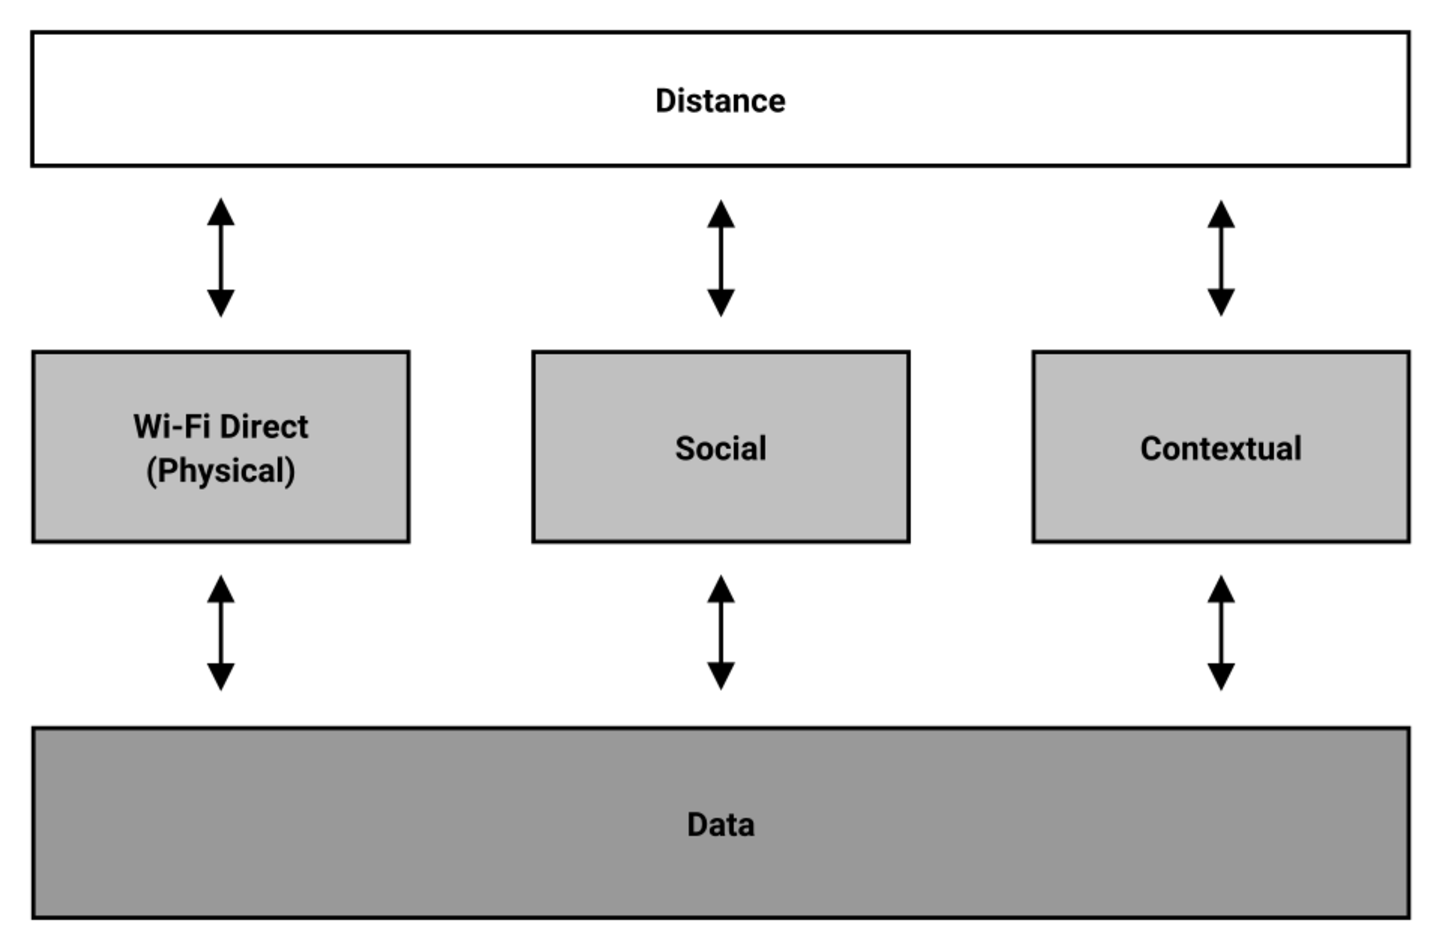
\includegraphics[width=\textwidth]{figures/fougere}
\end{frame}

\begin{frame}{Probabilistic Repartition}
    \begin{figure}
        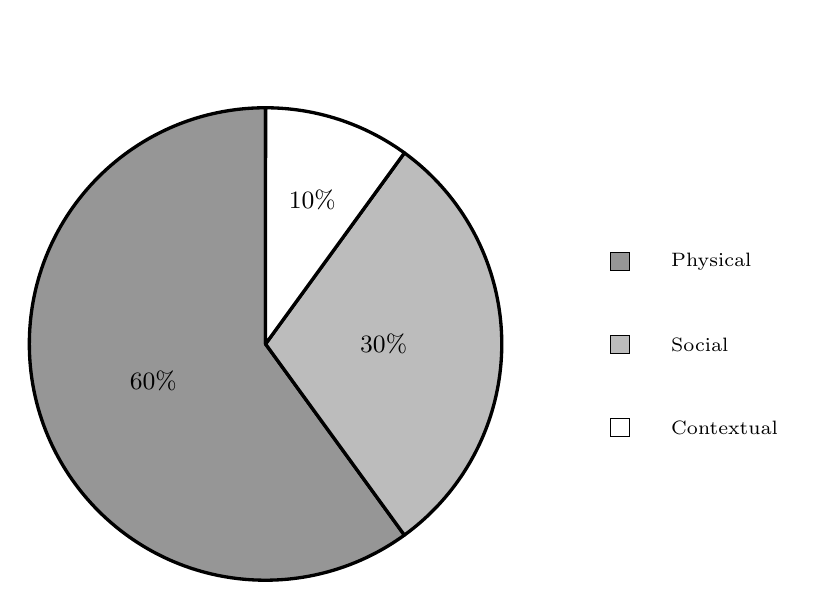
\begin{tikzpicture}
[
    pie chart,
    slice type={physical}{dgry},
    slice type={social}{lgry},
    slice type={contextual}{white},
    pie values/.style={font={\small}},
    scale=3
]

    \pie{}{60/physical,30/social,10/contextual}
    \legend[shift={(1.5cm,0.7cm)}]{{Physical}/physical, {Social}/social, {Contextual}/contextual}
\end{tikzpicture}
    \end{figure}
\end{frame}
